\documentclass[conference]{IEEEtran}
\IEEEoverridecommandlockouts
\usepackage{cite}
\usepackage{amsmath,amssymb,amsfonts}
\usepackage{algorithmic}
\usepackage{graphicx}
\usepackage{textcomp}
\usepackage{xcolor}
\usepackage{tabularx}
\usepackage{multirow}
\usepackage{graphics} % for pdf, bitmapped graphics files
\usepackage{subfig}
\usepackage{subcaption}
\usepackage{hyperref}
\usepackage{academicons}
\usepackage{xcolor}
\usepackage{listings}
\def\BibTeX{{\rm B\kern-.05em{\sc i\kern-.025em b}\kern-.08em
		T\kern-.1667em\lower.7ex\hbox{E}\kern-.125emX}}
% Gráficas en MATLAB
\usepackage{tikz, pgfplots}
% Color Enlace
\definecolor{colorEnlace}{RGB}{0, 0, 0}
\hypersetup{
	colorlinks=true,
	linkcolor=colorEnlace,
	citecolor=colorEnlace,
	urlcolor=colorEnlace,
	pdfauthor={Ruth Juana Espino Puma},
	pdftitle={}
}
% Control 
\usepackage{amsmath}
\begin{document}
	
	\title{Experiencia N°4 - Diseño de Controlador PID}
	
	\author{
		\IEEEauthorblockN{Ing. Darcy Arredondo Huarac}
		\IEEEauthorblockA{
			Laboratorio de Control I\\
			Cusco, Perú\\
			diego.arredondo@unsaac.edu.pe}
		\and
		\IEEEauthorblockN{Ruth Juana Espino Puma}
		\IEEEauthorblockA{
			Estudiante de Ingeniería Electrónica \\
			Cusco, Perú \\
			184657@unsaac.edu.pe}
		\and
		\IEEEauthorblockN{Davis Bremdow Salazar Roa}
		\IEEEauthorblockA{
			Estudiante de Ingeniería Electrónica \\
			Cusco, Perú \\
			200353@unsaac.edu.pe
		}
	}
	\maketitle
	
	\begin{abstract}
		The document outlines the design of a PID controller using the Ziegler-Nichols tuning method for an analog control system. The objectives include designing controllers for underdamped and overdamped cases, aiming to reduce overshoot and response time. For the underdamped case, calculations for parameters \( k_p \), \( k_i \), and \( k_d \) are based on a derived transfer function, with the system tuned to cut overshoot by half. For the overdamped case, similar calculations optimize response time. Simulations in MATLAB/Simulink demonstrate step and impulse responses, highlighting improvements in control. Additionally, the document presents PID circuit designs with specified resistor and capacitor values for each damping case, along with simulated output graphs for analysis.
	\end{abstract}
	
	\begin{IEEEkeywords}
		PID controller design, Ziegler-Nichols method, analog control system, underdamped response, overdamped response, transfer function, gain tuning, MATLAB/Simulink simulation, circuit design, response optimization
	\end{IEEEkeywords}
	\section{Procedimiento Experimental}
	Durante el procedimiento experimental se realizo la implementación de los circuitos para el control PID y planta de segundo orden como se define en \cite{ogata2015}, en la placa de pruebas o protoboard, las cuales en cada caso fueron alimentadas mediante una señal cuadrada, observando las salidas mediante el osciloscopio, las cuales se detallan en las figuras \ref{fig:sub-respuesta-general} y \ref{fig:sobre-respuesta-general}
	
	\begin{figure}[h]
		\centering
		\includegraphics[width=0.9\linewidth]{media/Implementación_Subamortiguado.jpg}
		\caption{Implementación PID caso subamortiguado}
		\label{fig:enter-label}
	\end{figure}
	
	\begin{figure}
		\centering
		\includegraphics[width=0.9\linewidth]{media/Implementación_Sobreamortiguado.jpg}
		\caption{Implementación PID caso sobreamortiguado}
		\label{fig:enter-label}
	\end{figure}
	\section{\textbf{Informe Final}}
	\subsection{\textbf{Muestre las gráficas obtenidas con el Osciloscopio para el caso Subamortiguado y Sobreamortiguado en lazo cerrado}}   
	
	\begin{figure}[h]
		\centering
		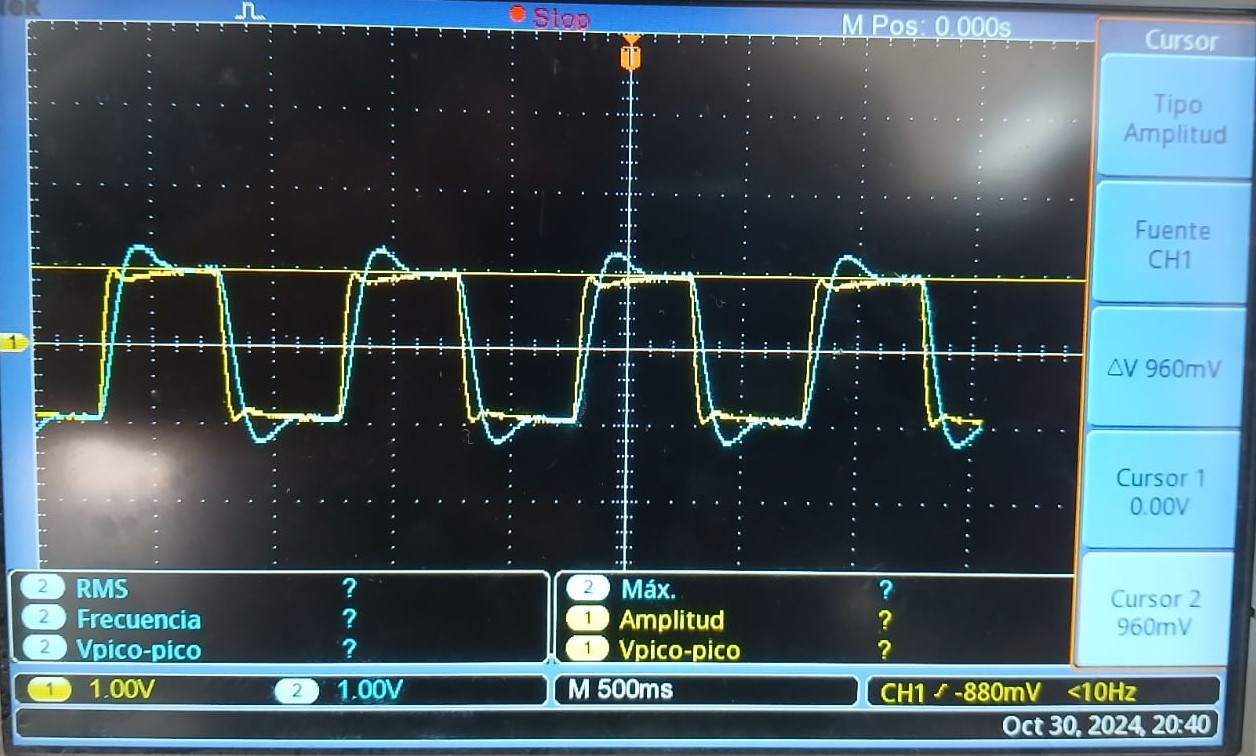
\includegraphics[width=0.4\textwidth]{media/sub-respuesta-general.jpeg}
		\caption{Comparación de la respuesta de respuestas PID - subamortiguado}
		\label{fig:sub-respuesta-general}
	\end{figure}
	
	\begin{figure}[h]
		\centering
		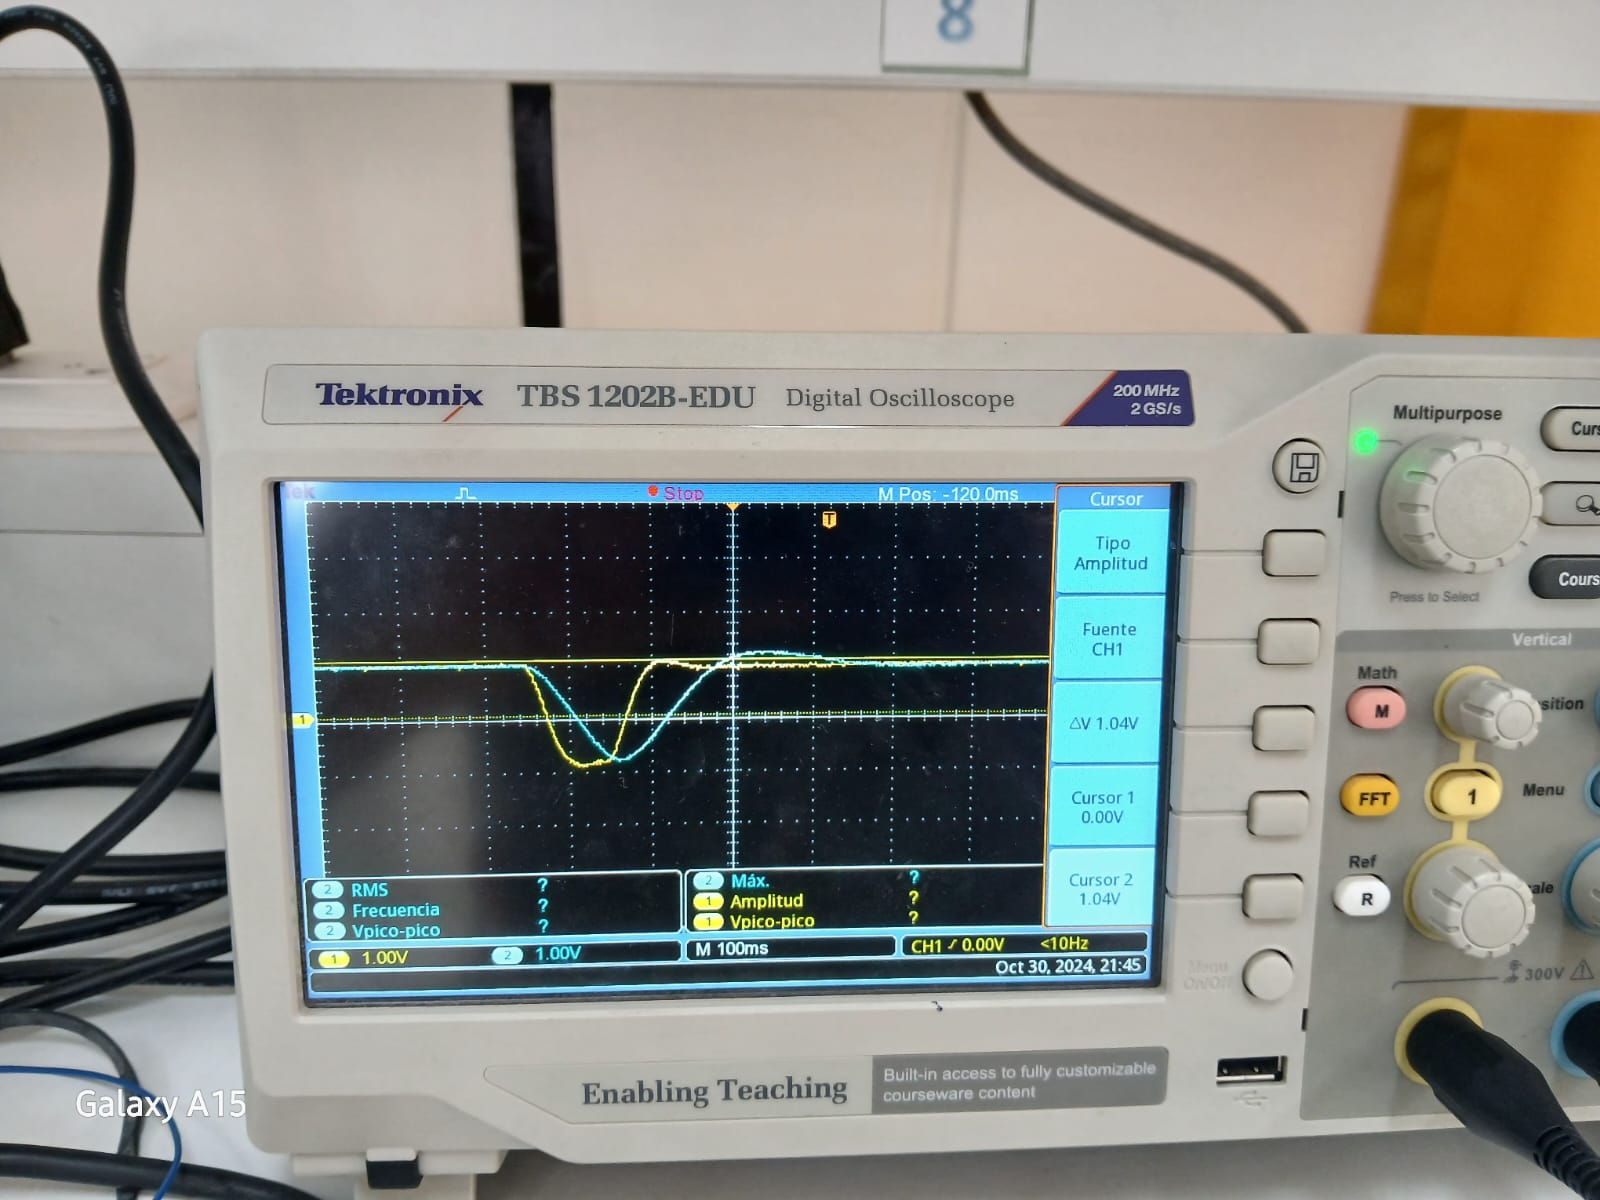
\includegraphics[width=0.4\textwidth]{media/sub-sobrepico-104.jpeg}
		\caption{Sobreimpulso del sistema subamortiguado - PID}
		\label{fig:sub-sobrepico-104}
	\end{figure}
	
	\begin{figure}[h]
		\centering
		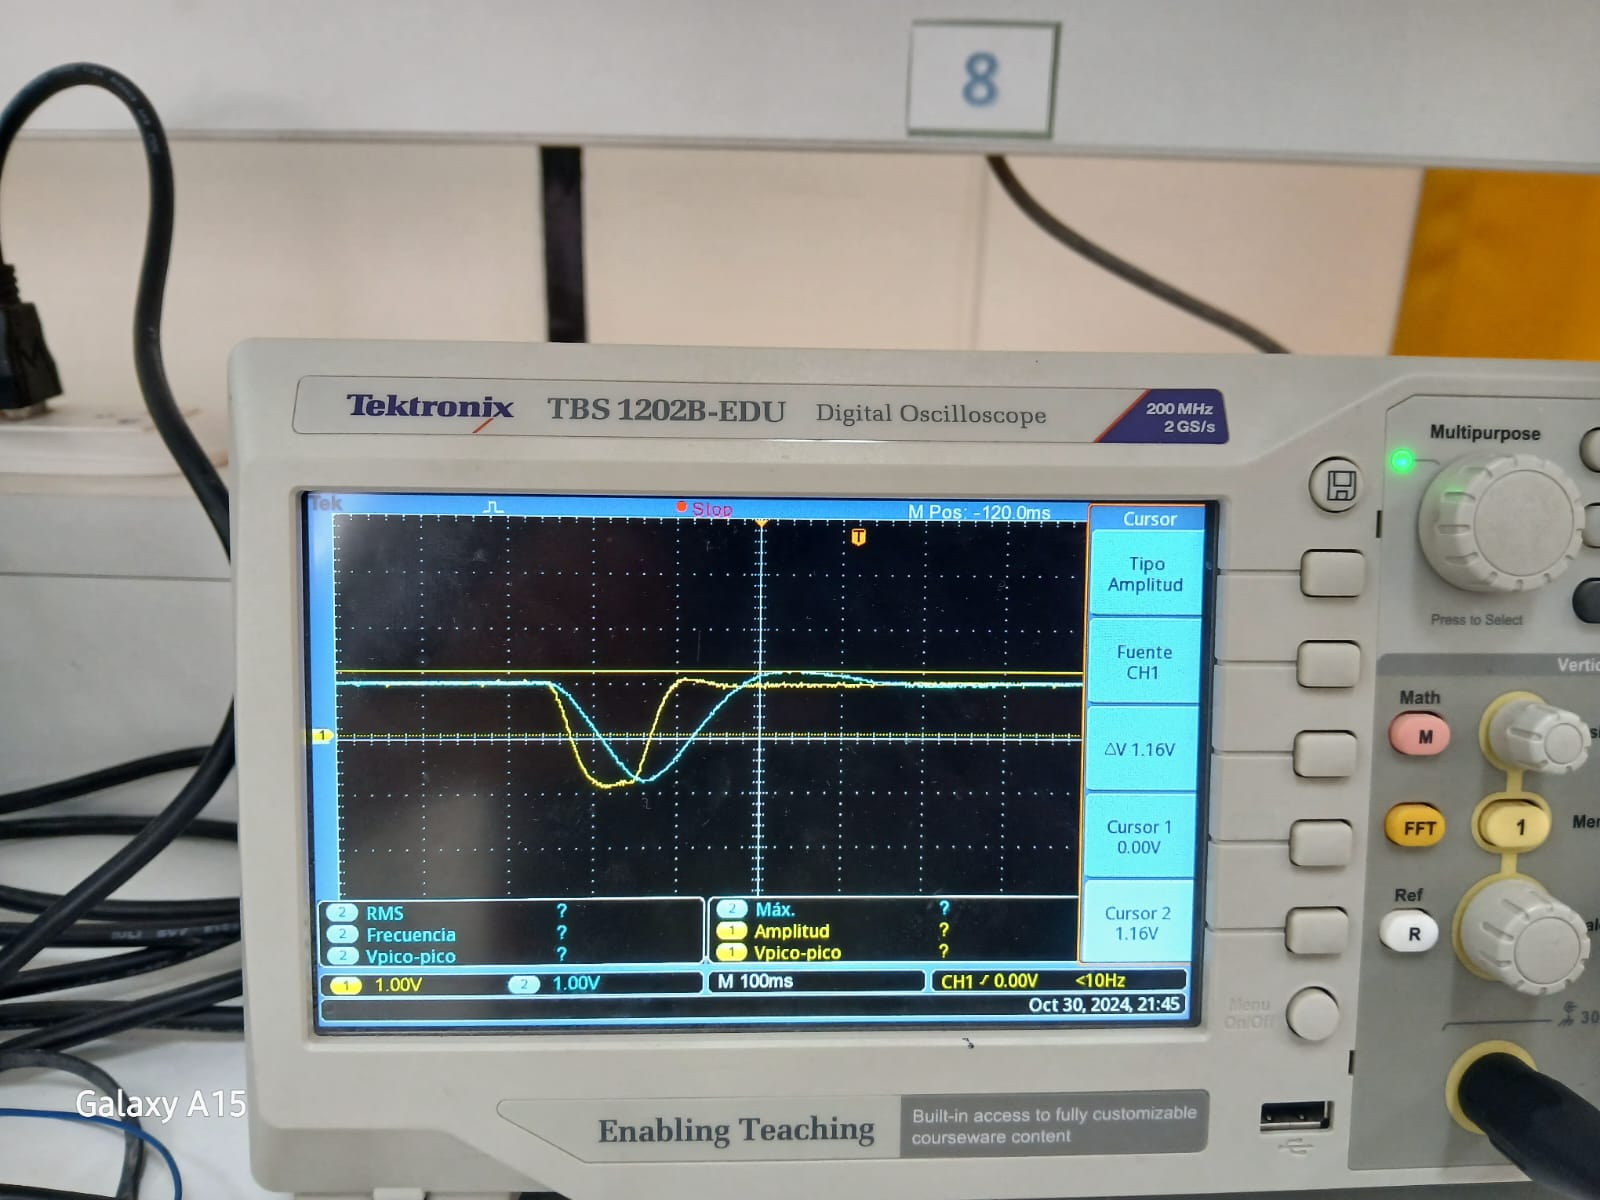
\includegraphics[width=0.4\textwidth]{media/sub-sobrepico-116.jpeg}
		\caption{Sobreimpulso del sistema subamortiguado sin PID}
		\label{fig:sub-sobrepico-116}
	\end{figure}
	
	En el caso sobreamortiguado la respuesta del sistema se aprecia en la figura
	
	\begin{figure}
		\centering
		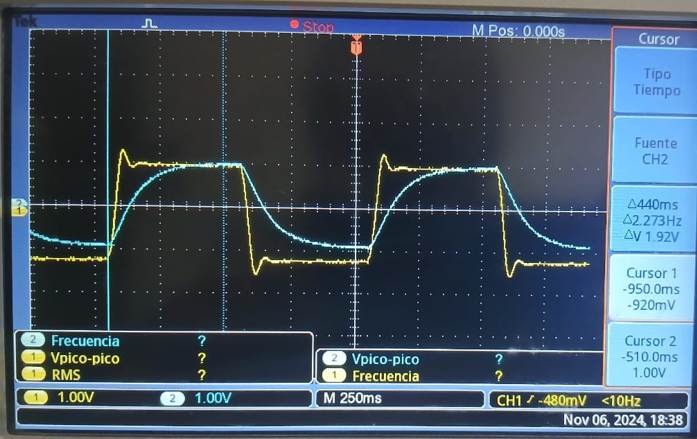
\includegraphics[width=0.5\textwidth]{media/sobre-respuesta-general.png}
		\caption{Comparación de respuestas PID - sobreamortiguado}
		\label{fig:sobre-respuesta-general}
	\end{figure}
	
	\begin{figure}
		\centering
		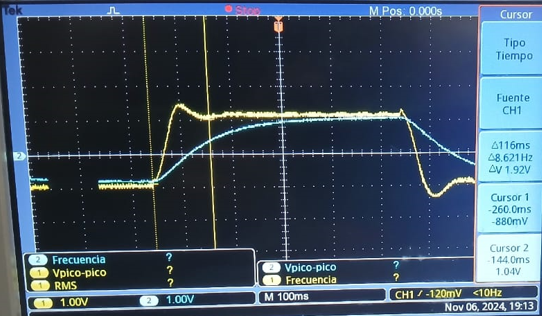
\includegraphics[width=0.9\linewidth]{media/sobre-ts-116.png}
		\caption{Reducción en el tiempo de establecimiento del sistema}
		\label{fig:sobre-ts-116}
	\end{figure}
	
	\subsection{\textbf{¿La respuesta hallada en forma teórica es igual o similar al circuito implementado?}}
	
	En la implementación para ambos casos (sistema subamortiguado y sobreamortiguado) la respuesta no fue la misma que la modelada teóricamente y simulada en NI Multisim, debido a 2 causas principales entre las cuales figuran la varibilidad en magnitud de los componente y/o materiales como las resistencias y capacitancias y el ruido generado por las fuentes de alimentación presentes al momento de implementar los circuitos.
	
	En la figura \ref{fig:sub-sobrepico-simulado} se puede apreciar la respuesta del sistema frente a una señal cuadrada siendo la señal de color verde la respuesta sin la compensación mediante PID y la naranja la señal de respuesta con el sobrepico disminuido al aplicar el control PID a la planta.
	\begin{figure}[h]
		\centering
		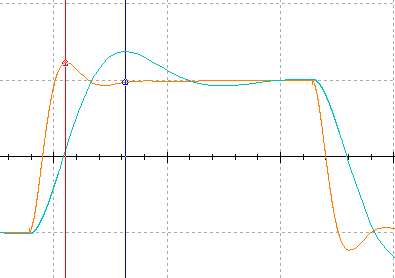
\includegraphics[width=0.5\textwidth]{media/sub-sobrepico-simulado}
		\caption{Respuesta del sistema subamortiguado en NI Multisim}
		\label{fig:sub-sobrepico-simulado}
	\end{figure}
	
	\begin{figure}
		\centering
		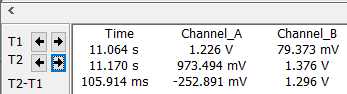
\includegraphics[width=0.5\textwidth]{media/medicion-sub-sobrepico-simulado.png}
		\caption{Valores medidos de amplitud del sobrepico para subamortiguado }
		\label{fig:emdicion-sub-sobrepico-simulado}
	\end{figure}
	
	\subsection{\textbf{Comente acerca del error de la señal de salida con respecto a la señal de entrada}}
	En un sistema de control retroalimentado, la señal de error es la diferencia entre la señal de referencia (o punto de referencia) y la señal de salida real del sistema, el propósito general es medir la distancia o diferencia entre el valor deseado y el valor actual de la variable que se está controlando, siendo así que esta variable para el sistema de control implementado es el voltaje, siendo así que el punto o señal de referencia se define como una magnitud relacionada a este parámetro y mediante la cual se limite la respuesta del sistema en función a este valor.
	
	\begin{figure}[h]
		\centering
		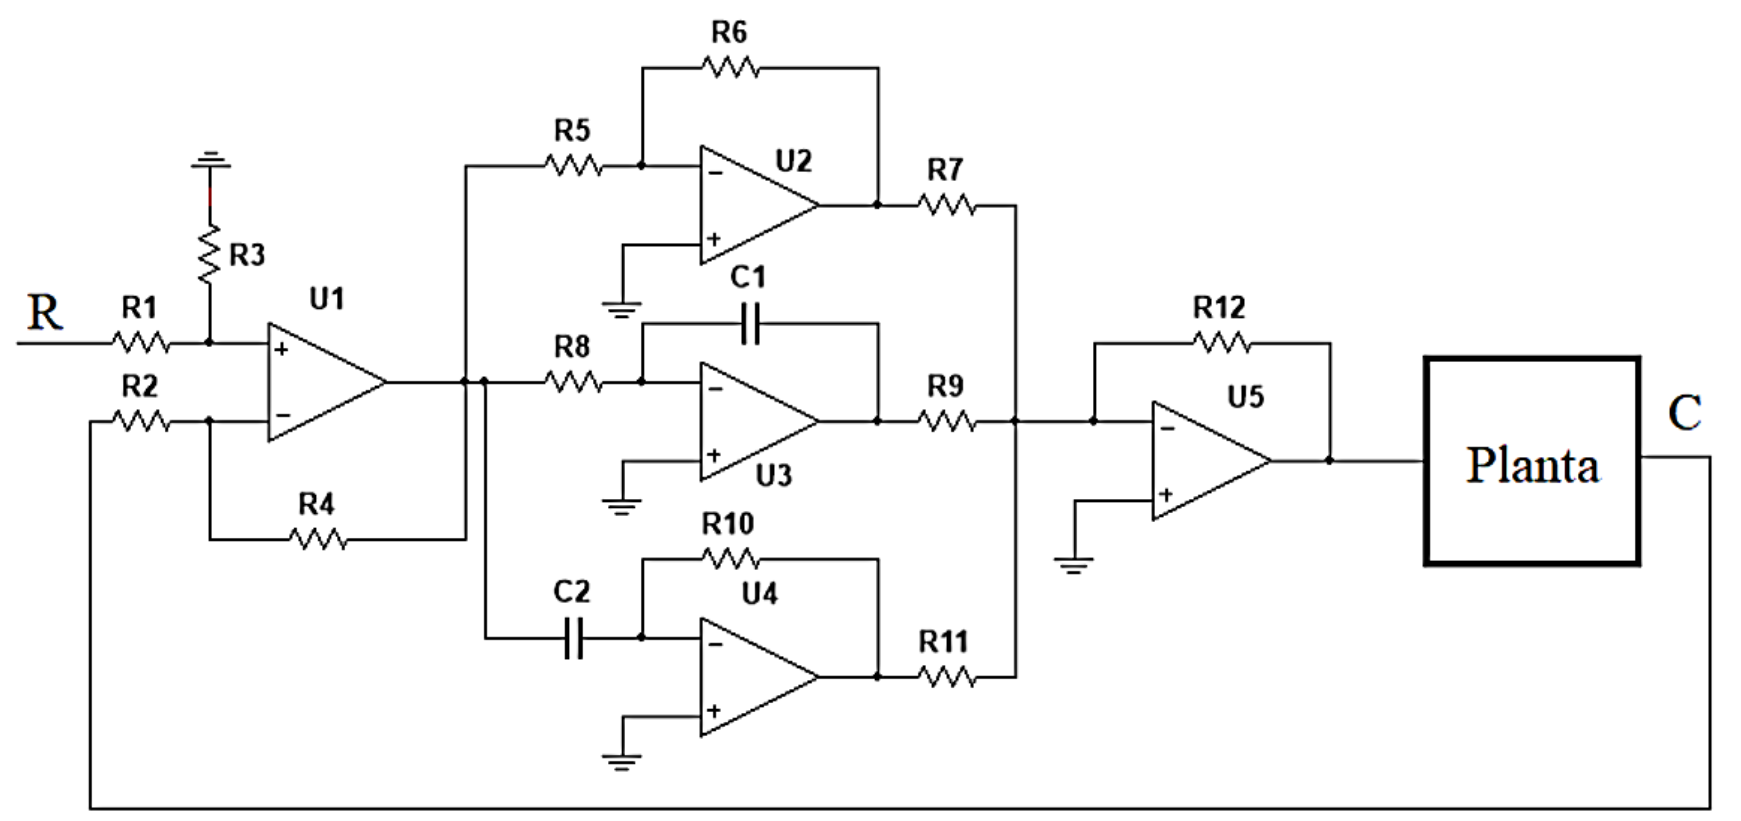
\includegraphics[width=0.5\textwidth]{media/esquematico-general.png}
		\caption{Esquema general para el control PID}
		\label{fig:esquematico-general}
	\end{figure}
	
	Para el modelado de los sistemas propuestas la señal de error en cada caso (sobre y sub amortiguado) se encuentra definida después del amplificador operacional U1 el cual esta configurado como restador teniendo como señal de referencia una señal cuadrada con un voltaje $V_{p} = 1v$ proveniente por el generador de funciones y la señal de salida proveniente de la planta que se realimenta por medio de la resistencia $R_2$ ingresando por el terminal negativo del amplificador operacional.
	
	Durante la experimentación mediante el software de simulación NI Multisim la señal de error para cada caso para un estado estable se muestra en la tabla \ref{tb:senal-error} y en la cual se muestra que la señal de error para el caso sobreamortiguado es menor en comparación a la señal de error del sistema subamortiguado.
	
	Lo que se justificar debido a que el sistema sobreamortiguado es más estable y cuenta con menos oscilaciones antes de llegar a su estabilidad
	las realidades de las personas que desean hacer algo al respecto ps de eso depende su vida con el resto de individuos en una sociedad
	
	\begin{table}[]
		\centering
		\caption{}
		\label{tb:senal-error}
		\begin{tabular}{|l|c|}
			\hline
			\multicolumn{1}{|c|}{\textbf{Tipo de Sistema}} & \textbf{Error {[}mV{]}} \\ \hline
			SubAmortiguado                                 & 365.526                 \\ \hline
			SobreAmortiguado                               & 357.351                 \\ \hline
		\end{tabular}
	\end{table}
	
	\section{Conclusiones}
	La implementación del controlador PID, usando el método de sintonización de Ziegler-Nichols, mejoró notablemente las respuestas del sistema en casos subamortiguados y sobreamortiguados. En el caso subamortiguado, se logró reducir el sobreimpulso a la mitad, mientras que en el caso sobreamortiguado se optimizó el tiempo de respuesta. Los resultados simulados en MATLAB/Simulink confirmaron estas mejoras, mostrando una disminución en el sobreimpulso y una respuesta más rápida y estable en ambos escenarios, lo cual valida la efectividad del diseño y sintonización aplicados.
	
	A pesar de los resultados teóricos y simulados, el comportamiento del circuito implementado en la protoboard mostró discrepancias debido a factores como la variabilidad de los componentes y el ruido de las fuentes de alimentación. En las pruebas, se observó que el sistema sobreamortiguado presentó un menor error en comparación con el sistema subamortiguado, reflejando una mayor estabilidad y menos oscilaciones antes de alcanzar el estado estable. Esto evidencia la influencia de las condiciones prácticas en la respuesta real del sistema PID, destacando la importancia de considerar estos factores en aplicaciones reales.
	
	
	
	\bibliographystyle{IEEEtran}
	\bibliography{biblio}
\end{document}